\documentclass[11pt]{article}
\usepackage{float}
\usepackage[portuges]{babel}%Babel -- irá activar automaticamente as regras apropriadas de hifenização para a língua todo o
                                   %-- o texto gerado é automaticamente traduzido para Português.
                                   %  Por exemplo, “chapter” irá passar a “capítulo”, “table of contents” a “conteúdo”.
                                   % portuges -- específica para o Português.
\usepackage[utf8]{inputenc} % define o encoding usado texto fonte (input)--usual "utf8" ou "latin1
\usepackage[T1]{fontenc}
\usepackage{graphicx}
%\usepackage{layout}

%used to fix header space
\usepackage[headheight=0pt,headsep=0pt]{geometry}
\addtolength{\topmargin}{-40pt}
\addtolength{\textheight}{120pt}

\usepackage{tabularx}

\title{Laboratórios de Informática III \\
       \textbf{Trabalho Prático C}\\ Relatório de Desenvolvimento
       } %Titulo do documento
\author{Pedro Costa\\ (a85700) \and Miguel Caravalho\\ (A84518)
         \and Maria João Moreira\\ (A89540)
       } %autores do documento
\date{06-04-2020} %data


\begin{document}
\begin{titlepage}
    
\includegraphics[width=\columnwidth]{images/capa.pdf}
\end{titlepage}
\newpage

\newpage
\tableofcontents %insere o índice

\newpage
\section{Introdução}
Mantém-se tudo o que foi dito na introdução do projeto de C. Em suma, continuamos a querer explorar os conhecimentos adquiridos noutras UC's e, a partir dos mesmos, desenvolver estruturadamente uma aplicação de média escala com conceitos que se adequem à dimensão. Mudamos agora a linguagem para o efeito. O paradigma mantém-se dentro de orientado aos objectos, agora numa linguagem que realmente é feita para tal, Java. 

Desta vez, iremos tirar partido dos princípios da programação com interfaces que nos irá permitir ter um projeto extremamente flexível, como se fosse um puzzle composto por várias peças. A grande vantagem de tamanha flexibilidade é que podemos trocar peças do puzzle à vontade, desde que tenham o mesmo formato (neste caso, a mesma interface).

\newpage
\section{Módulos e funcionalidades correspondentes}

\subsection{Packages principais do GestVendasModel - Visão superficial}
O módulo principal da nossa aplicação, o \textbf{GestVendasModel} foi desenvolvido à volta dos seguintes packages em que cada armazena um módulo independente:

\begin{itemize}
    \item \textbf{Base}: Este package contém definições para as entidades base de todo o sistema, ou seja, produtos, clientes e vendas. Ainda que algumas destas entidades pudessem ser representadas atomicamente, decidimos encapsulá-las numa interface própria.
    \item \textbf{Catalogs}: Neste package estão presentes as representações do Catálogo de Produtos e do Catálogo de Clientes, dois dos módulos principais que compoem o GestVendasModel.
    \item \textbf{Billing}: Package que contém toda a informação relativa ao módulo de dados da faturação. A faturação por sua vez é um módulo de dados que relaciona produtos com informação relativa às suas vendas.
    \item \textbf{Branch}: Package que contém toda a informação relativa ao módulo de dados que representa uma filial. Uma filial, por usa vez, é um módulo de dados que relaciona clientes com os produtos que compram para \textbf{uma} dada filial.
    \item \textbf{Configs e Statistics}: Package que armazena módulos de configurações e estatisticas relativas a um GestVendasModel.
    \item \textbf{Parsers}: Neste package define-se as condições de um parser capaz de carregar um GestVendasModel a partir dos ficheiros de produtos, clientes e vendas fornecidos.
\end{itemize}

\vspace{1cm}
\begin{figure}[h]
    \centering
    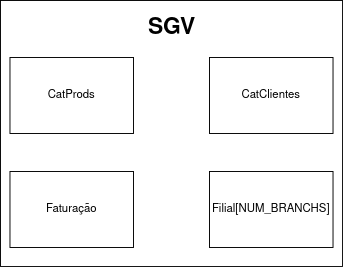
\includegraphics[width=\textwidth,height=5cm]{images/sgv.png}
    \caption{Componentes do SGV}
\end{figure}

\newpage
\subsubsection{Package Base}
Neste package, como explicado anteriormente, guardam-se as interfaces e respetivas implementações das entidades Produto, Cliente e Venda.
Ao encapsular os produtos e os clientes (que podiam ser representados atomicamente por uma String) numa interface própria permitimos que, num futuro indeterminado, fosse simples adicionar novos tipos de produtos/clientes mais complexos que não pudessem ser representados atomicamente, sem necessitar de fazer alterações em mais lado nenhum.

\subsubsection{Package de Catálogos}
Neste package definem-se apenas as interfaces e classes do que são catálogos de produtos e clientes. A interface de ambos é praticamente igual diferindo apenas no facto de armazenar produtos ou clientes.

Permite verificar se existe um produto no catálogo e, obviamente, permite que sejam inseridos no mesmo. Além disso é ainda capaz de nos informar acerca do numero de entradas que contém.  
\subsubsection{Package Billing}
Este package contém todas as interfaces, e respetivas implementações em classes, necessárias para se definir o conceito de Faturação. Como indicado anteriormente, aqui guardam-se relações entre produtos e as suas vendas.

A interface da faturação oferece várias operações distintas começando por permitir faturar vendas, verificar se produtos foram vendidos (e obter a sua informação), obter todos os produtos não vendidos, entre várias outras funcionalidades.

Para esse efeito, encapsulamos todos os dados de vendas dum produto num módulo próprio, sendo esse o \textbf{ProductInfo}. Assim, o nosso módulo faturação define apenas um \textbf{mapeamento entre produtos e a sua informação}. Tiramos ainda partido de algumas variáveis auxiliares para acumular informação que sabemos que será útil, como se pode ver abaixo.
\begin{verbatim}
    private Map<IProduct, IProductInfo> billing;
    private float totalBilled;
    private int[][] globalNumberOfSales;
    private int number_of_branches;
    private int number_of_months;
    private int number_of_types; 
\end{verbatim}
\vspace{1cm}
\begin{figure}[H]
    \centering
    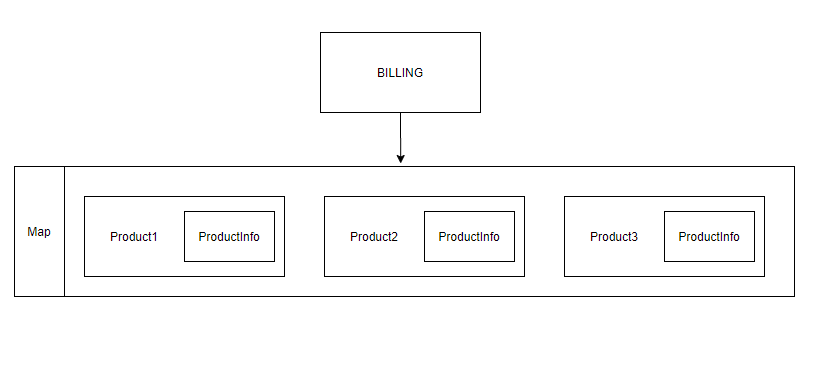
\includegraphics[width=\textwidth,height=10cm]{images/esquema_billing.png}
    \caption{\textbf{Esquema do módulo Billing}}
\end{figure}

\subsubsection{Package Branch}
Este package contém todas as interfaces, e respetivas implementações em classes, necessárias para se definir o conceito de Filial. Como indicado anteriormente, aqui guardam-se relações entre clientes e os produtos comprados pelos mesmos.

A interface da filial oferece várias operações distintas começando por permitir assinalar que um cliente comprou um determinado produto, verificar quantos compradores distintos houve num determinado mês, obter toda a informação relativa às compras de um cliente, obter o total gasto pelos clientes na filial, entre várias outras operçaões.

Para obter este efeito, encapsulamos todo o historial de compras de cada cliente numa estrutura própria a que chamamos de \textbf{ProductsBought}. Aqui temos um mapeamento entre todos os produtos comprados por um determinado cliente e a informação acumulada dos mesmos (encapsulada por sua vez numa outra estrutura apelidada de \textbf{CustomerBought}). Tiramos ainda partido de algumas variáveis auxiliares que nos permitiram acumular informação útil numa fase mais avançada, evitando assim procuras desnecessárias mais tarde.

\begin{verbatim}
    private Map<ICustomer, IProductsBought> branch;
    private int[] distinctCustomers;
    private int number_of_months; 
\end{verbatim}

\vspace{1cm}
\begin{figure}[H]
    \centering
    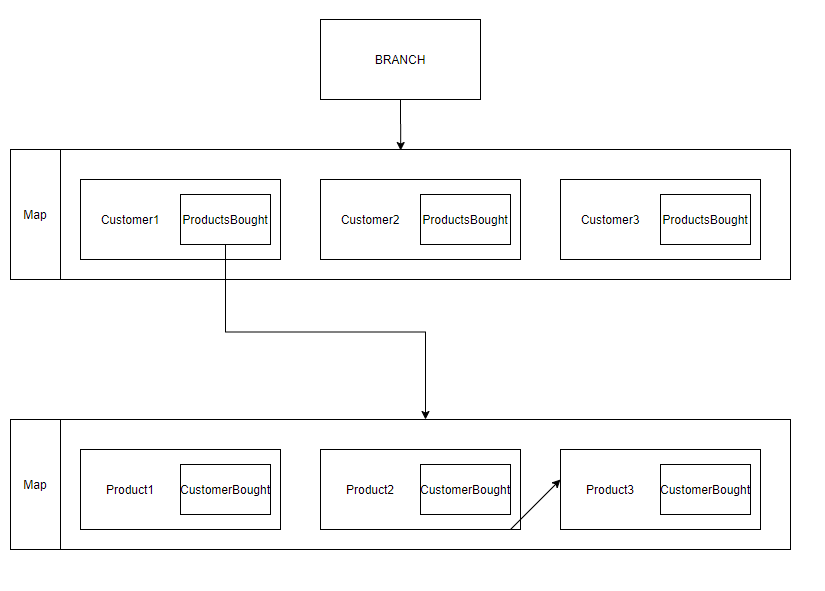
\includegraphics[width=\textwidth,height=10cm]{images/esquema_branch.png}
    \caption{\textbf{Esquema de uma Branch}}
\end{figure}
\subsubsection{Package de parsers}
Neste package define-se a interface que caracteriza os requisitos mínimos de um parser. A partir daí definimos dois parsers "completos". Um parser que utiliza o package \textit{nio} e lê o ficheiro como uma stream, um outro parser que utiliza um \textit{BufferedReader}.

Além destes, apenas com o propósito de cumprir os testes de performance pedidos, foram desenvolvidos mais seis parsers (três com \textit{streams} e três com \textit{BufferedReader} para fazer parse de todos os ficheiros nos seguintes três cenários:
\begin{itemize}
    \item \textbf{Sem fazer parse}: Apenas percorrer as linhas dos ficheiro de vendas sem fazer absolutamente nada.
    \item \textbf{Sem validação}: Percorrer as linhas dos ficheiro de vendas e construir a estrutura que contém a venda, sem ver se se trata de uma venda válida ou inválida.
    \item \textbf{Com validação e parsing}: Percorrer as linhas dos ficheiros de vendas e construir a estrutura que contém uma venda, assim como ver se esta é válida.
\end{itemize}

Além desses seis, foram ainda desenvolvidos mais quatro parsers (capazes de cumprir os propósitos acima e também fazer parse normalmente, inserindo nas estruturas de dados as vendas). Estes servem para realizar um dos testes de performance pedidos que se aplica apenas ao ficheiro \textit{Vendas\_5M.txt} e onde são utilizadas \textit{streams} \textbf{paralelas}.

\subsubsection{Package de Configs e Statistics}
Este package contém as interfaces e respetivas implementações para dois módulos importantes do GestVendasModel.

O primeiro, \textbf{Configs}, contém o conjunto de dados iniciais com o qual vamos trabalhar. Isto compreende um conjunto de dados como o número de filiais que temos, onde se localizam os ficheiros que queremos ler, entre vários outros campos.

O segundo, \textbf{Statistics}, armazena alguma informação que foi utilizada para responder às queries estatísticas como o número total de vendas, a quantidade de vendas válidas, a quantidade de vendasa com valor zero, entre outros.
\newpage

\subsection{Outros packages desenvolvidos por necessidade/utilidade} 
\subsubsection{Navegador}
Este package pertence efetivamente ao conjunto de packages do \textit{model} mas como não é uma peça utilizada diretamente no mesmo não foi abordado acima.

Desta vez houve, em comparação com o projeto anterior, um investimento muito maior no módulo \textbf{Navigator} por parte do grupo. Quisemos desenvolver algo estruturado e bem dividido pelo que concluímos que um navegador pode ser abordado em três partes importantes e distintas:

\begin{itemize}
    \item \textbf{Página}: Como seria de esperar, o \textbf{Navigator} vai percorrer um conjunto de páginas, cada uma contendo uma porção da informação total que queremos demonstrar. Assim, desenvolvemos uma estrutura que encapsula cada página, o módulo \textbf{Page}.
    \item \textbf{Barra de estado}: Um dos problemas que tivemos com este módulo anteriormente foi a falta de comunicação com o utilizador. Assim, definimos uma barra de estado que, consoante o input do utilizador, varia para oferecer comentários e informação útil. Esta funcionalidade foi também encapsulada independentemente numa estrutura que apelidamos de \textbf{StatusBar}.
    \item \textbf{Navigator}: Claramente só falta unificar os módulos acima e temos a solução desejada. O \textbf{Navigator} é o responsável por guardar um conjunto de várias páginas e uma barra de estado. Define uma API capaz de fazer procuras de expressões regulares ao longo dos dados e navegar sobre as procuras, mudar de página (saltar ou movimentar para a frente ou para trás), dar setup a mensagens de erro para avisar o utilizador quando o input não é reconhecido, entre outras funcionalidades.
\end{itemize}

O navegador \textbf{não dá} display a informação por si só, é apenas um módulo que armazena informação e permite recolher o correspondente à página atual numa determinada estrutura, sendo assim uma componente do \textit{model} e não da \textit{view}.


\newpage
\subsubsection{Package Exceptions}
Neste package definem-se várias exceções utilizadas para avisar o utilizador com detalhe do que está a fazer de forma errada, ou desconhecida ao sistema, em qualquer interação.

\subsubsection{Package Controller}
Neste package encontra-se a interface e a implementação de um controlador que serve de ponte entre o utilizador e a camada de dados, \textit{model}, controlando também o que é mostrado ao utilizador a partir da \textit{view}. Iremos falar com detalhe da arquitetura MVC utilizada brevemente.

\subsubsection{Package View}
Tal como o anterior, guarda-se aqui a interface e a implementação de uma vista que permite demonstrar informação pré-determinada ao utilizador.

\subsubsection{Package Utilities}
Aqui guardam-se utilidades de natureza diferente. Temos o módulo \textbf{Crono} fornecido pelos professores, temos um módulo \textbf{Utilities} que têm apenas o propósito de compor caminhos de maneira a que funcione em Mac e Windows e, temos ainda, uma implementação de um par mutável \textbf{MutablePair} que foi extremamente útil numa situação pontual.

\subsubsection{Package Testing}
Nada neste package é utilizada com o objetivo de desenvolver a aplicação final GestVendasApp. Aqui guarda-se apenas um conjunto de programas externos que fazem \textit{logging} de dados pedidos na secção de medidas de performance.

\subsubsection{Encapsulamento}
Tal como pedido, garantimos que toda a informação fornecida em qualquer momento é apropriadamente clonada. Assim, garantimos a privacidade dos nossos módulos cuja implementação interna não tem de ser conhecida por ninguém. Além disso, as API's definidas tentam ser tão sucintas quanto possível, evitando deixar fugir detalhes sobre a implementação em qualquer momento.

\newpage
\section{Arquitetura da aplicação}
Mais uma vez, e como seria de esperar, utilizamos, para controlar a interação com o utilizador, uma arquitetura MVC em particular. Nesta, é de notar que há uma separação clara de conceitos entre as várias componentes. Eis o papel que cada um assume:
\begin{itemize}
    \item \textbf{Model}: A camada de dados trata apenas de lidar diretamente com dados que recebe ou com os dados que já contém. É capaz de responder a todas as necessidades de um programador que utilize este módulo, de forma genérica. Ou seja, conseguimos devolver todos os conjuntos de dados de forma que depois o programador pode manipular sem grande esforço para obter respostas mais especifícas (nesta secção não vamos ordenar dados por um critério por exemplo).
    \item \textbf{Controller}: O controlador age um pouco, como se pode confirmar na figura abaixo, como um \textit{Man in the middle}. Este vai receber todos os dados do utilizador, passá-los ao \textit{model} para receber a informação que precisa de volta, dar-lhe alguns tweaks caso seja necessário e, de seguida, envia a informação alterada para a \textit{view} para ser demonstrada ao utilizador de uma forma que apenas a própria \textit{view} conhece.
    \item \textbf{View}: A vista tem apenas o objetivo de receber dados de um certo tipo e dar-lhes display de uma forma qualquer. Neste projeto tudo se resume a texto num terminal, mas seria relativamente fácil, devido à modularidade e à arquitetura que temos, migrar as vistas para uma página web, por exemplo.
\end{itemize}

\vspace{1cm}
\begin{figure}[h]
    \centering
    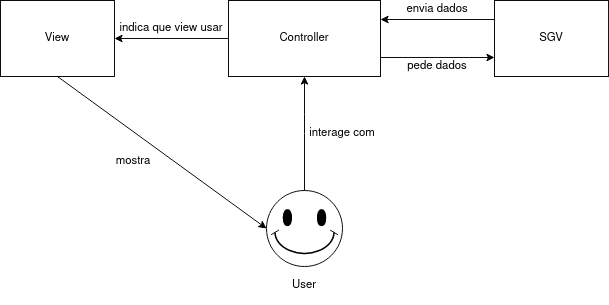
\includegraphics[width=\textwidth,height=10cm]{images/mvc.png}
    \caption{\textbf{Design pattern - MVC}}
\end{figure}

\newpage
\section{Medidas de performance}
Um aspeto pedido nesta fase do projeto não pedido anteriormente foi que se fizesse um conjunto de programas auxiliares para medir a performance em alguns cenários. Desenvolvemos os programas auxiliares e obtemos os seguintes resultados.

\subsection{Tempo de cada query}
Esta não foi uma das medidas pedidas mas tomamos a liberdade de criar um programa externo para extrair estes mesmos dados de forma simples. Eis o obtido.

\begin{figure}[h]
    \centering
    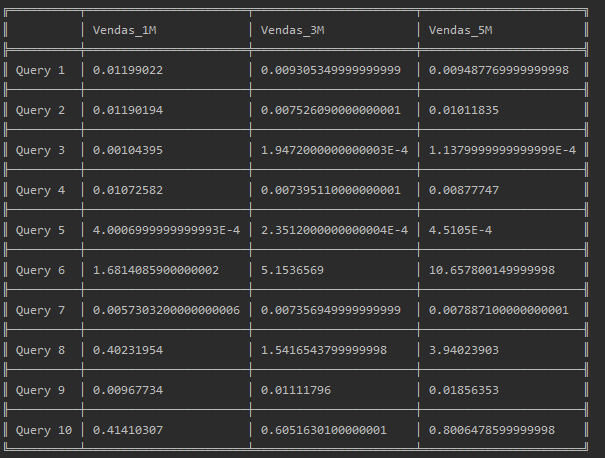
\includegraphics[width=\textwidth,height=10cm]{images/query_times.png}
    \caption{\textbf{Tempo médio obtido para cada query ao fim de 10 execuções.}}
\end{figure}

\textbf{Nota}: O computador utilizado para testes encontrava-se inundado de outras operações em simultâneo pelo que os teus tempos estão muito provavelmente inflacionados.

\subsection{Tópicos 1, 2 e 3 das medidas de performance pedidas}
Nestes tópicos pedia-se uma análise do tempo de parsing dos ficheiros de vendas utilizando BufferedReader (\textbf{BR}) e comparando com o uso do package \textit{nio} que utiliza \textbf{streams} para ler o ficheiro. Pretendia-se comparar 3 circunstâncias diferentes, sendo estas:

\begin{itemize}
    \item \textbf{NO\_PV}: Sem parsing nem validação (apenas percorrer as linhas).
    \item \textbf{P\_NO\_V}: Com parsing mas sem validação (percorrer as linhas e criar as estruturas das vendas, sem as validar).
    \item \textbf{PV}: Com parsing e validação.
    \item \textbf{FP}: Full parse, ou seja, parsing, validações e inserções nas estruturas de dados.
\end{itemize}

Apresentamos então os resultados obtidos num formato de tabela.

\vspace{0.5cm}
\begin{tabularx}{\textwidth} {
  | >{\centering\arraybackslash}X
  | >{\centering\arraybackslash}X
  | >{\centering\arraybackslash}X
  | >{\centering\arraybackslash}X
  | >{\centering\arraybackslash}X | }
    \hline
     & Vendas\_1M  & Vendas\_3M  & Vendas\_5M  \\
    \hline
    NIO\_NO\_PV & 0.139s & 0.426s & 0.702s  \\
    \hline
    NIO\_P\_NO\_V & 0.474s & 1.403s & 2.109s \\
    \hline
    NIO\_PV & 0.707s & 2.145s & 3.667s \\
    \hline
    NIO\_FP & 2.278s & 8.423s & 14.746s \\
    \hline
    BR\_NO\_PV & 0.132s & 0.419s & 0.666s  \\
    \hline
    BR\_P\_NO\_V & 0.425s & 1.239s & 2.056s \\
    \hline
    BR\_PV & 0.684s & 2s & 3.356s \\
    \hline
    BR\_FP & 2.346s & 8.267s & 14.319s \\
    \hline
\end{tabularx}
\vspace{0.5cm}

Como podemos ver pela tabela acima, os tempos crescem (entre \textbf{NIO} ou entre \textbf{BR}) de forma constante consoante o input aumenta de tamanho. É de notar que o uso de \textbf{BufferedReader} obteve praticamente sempre tempos superiores ao uso de \textbf{Streams} possivelmente devido a não estarmos a usar um grande volume de dados ou, ainda mais provável, por estarmos a fazer um conjunto bastante pequeno de operações sobre os dados. As streams "benificiam" de muitas operações sobre o conjunto de dados na totalidade.

Apresentamos ainda os resultados obtidos de forma gráfica:
\begin{figure}[H]
    \centering
    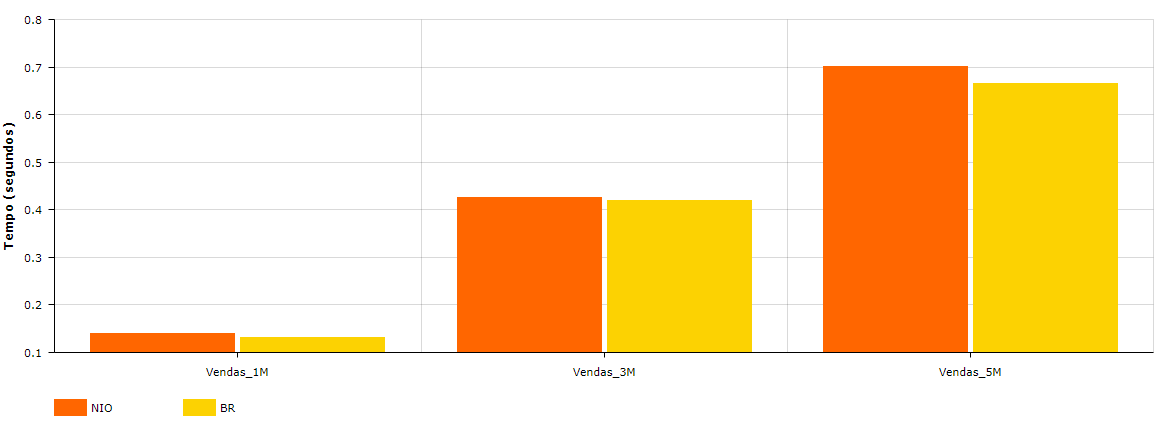
\includegraphics[width=\textwidth,height=10cm]{images/nio_vs_br_no_pv.png}
    \caption{\textbf{Resultados obtidos para o cenário sem parsing nem validação}}
\end{figure}
\begin{figure}[H]
    \centering
    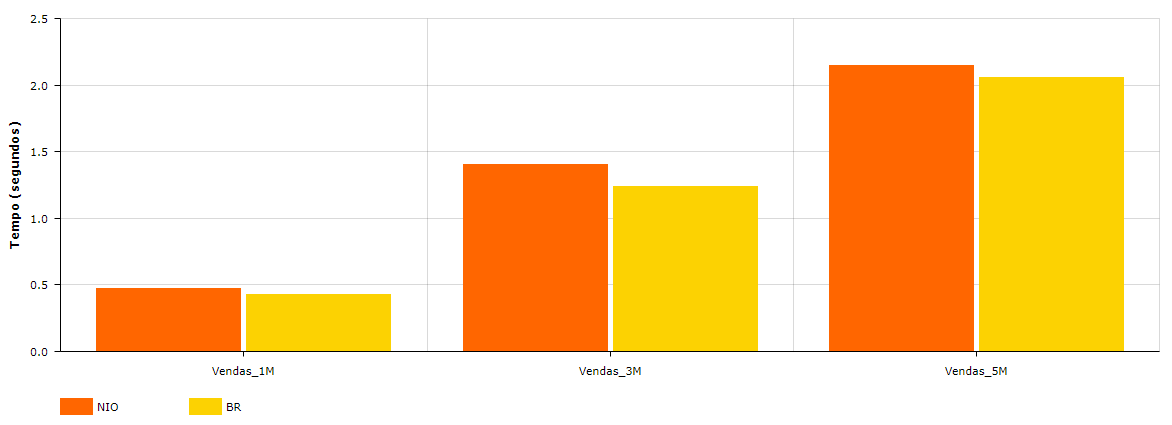
\includegraphics[width=\textwidth,height=10cm]{images/nio_vs_br_p_no_v.png}
    \caption{\textbf{Resultados obtidos para o cenário com parsing e sem validação}}
\end{figure}
\begin{figure}[H]
    \centering
    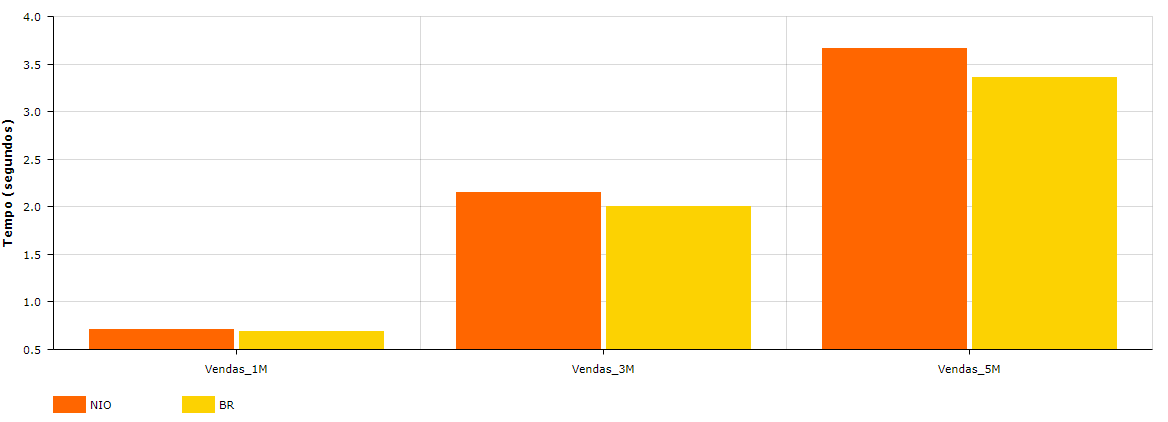
\includegraphics[width=\textwidth,height=10cm]{images/nio_vs_br_pv.png}
    \caption{\textbf{Resultados obtidos para o cenário com parsing e validação}}
\end{figure}
\begin{figure}[H]
    \centering
    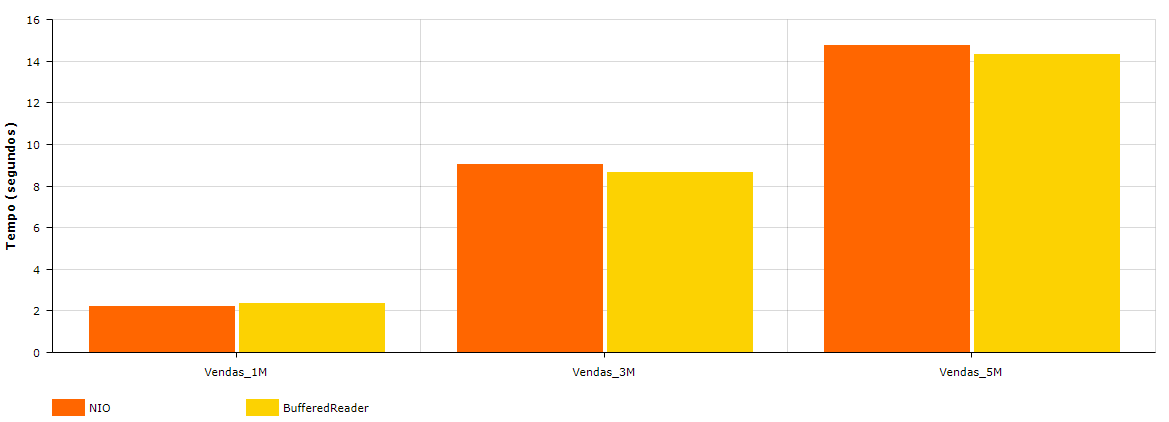
\includegraphics[width=\textwidth,height=10cm]{images/nio_vs_br_full_parse.png}
    \caption{\textbf{Resultados obtidos para o cenário com parsing e validação}}
\end{figure}

\newpage

\subsection{Medições das queries 5 à 9 com implementações diferentes}
Neste tópico era pedido que se atuasse sobre as queries 5 à 9. O que se pedia em concreto era apenas que variássemos dentro das possíveis implementações de \textbf{Set}, \textbf{Map} e \textbf{List} consoante o que estivessemos a usar. 

No nosso caso, todas essas queries utilizavam apenas um \textbf{Map} pelo que alternamos entre implementações com \textbf{HashMap} e com \textbf{TreeMap}.
 
\vspace{0.5cm}
\begin{tabularx}{\textwidth} {
  | >{\centering\arraybackslash}X
  | >{\centering\arraybackslash}X
  | >{\centering\arraybackslash}X
  | >{\centering\arraybackslash}X
  | >{\centering\arraybackslash}X | }
    \hline
     & Vendas\_1M  & Vendas\_3M  & Vendas\_5M  \\
    \hline
    Query 5 & 0.0004s & 0.0006s & 0.0007s \\ 
    \hline
    Query 6 & 1.341s & 4.012s & 7.404s  \\
    \hline
    Query 7 & 0.007s & 0.008s & 0.009s \\
    \hline
    Query 8 & 0.401s & 1.523s & 3.763s \\
    \hline
    Query 9 & 0.011s & 0.012s & 0.014s  \\
    \hline
\end{tabularx}
\textbf{Legenda}: Resultados obtidos com \textbf{HashMap}.
 
\vspace{0.5cm}
\begin{tabularx}{\textwidth} {
  | >{\centering\arraybackslash}X
  | >{\centering\arraybackslash}X
  | >{\centering\arraybackslash}X
  | >{\centering\arraybackslash}X
  | >{\centering\arraybackslash}X | }
    \hline
     & Vendas\_1M  & Vendas\_3M  & Vendas\_5M  \\
    \hline
    Query 5 & 0.0006s & 0.001s & 0.001s \\ 
    \hline
    Query 6 & 1.632s & 4.587s & 9.871s  \\
    \hline
    Query 7 & 0.007s & 0.010s & 0.009s \\
    \hline
    Query 8 0.403s& s & 1.705s & 4.064s \\
    \hline
    Query 9 & 0.012s & 0.012s & 0.012s  \\
    \hline
\end{tabularx}
\textbf{Legenda}: Resultados obtidos com \textbf{TreeMap}.
\vspace{0.5cm}

Nota-se então que, para queries mais pesadas, usar o \textbf{TreeMap} traz uma grande perda de eficiência. Isto seria expetável uma vez que a vantagem do \textbf{TreeMap} é permitir inserções de acordo com um certo critério, algo que não nos importa em nenhuma destas queries.

\subsection{Medições relativas a Parallel Streams}
Uma outra medição que foi pedida era relativa a fazer parsing do ficheiro de vendas com 5 milhões de linhas utilizando \textbf{Streams paralelas}. Consideramos os mesmos cenários da secção \textbf{4.2} e um cenário adicional em que fazemos o parsing total (inserindo a informação nas estruturas de dados).

Obtivemos os seguintes resultados:

\vspace{0.5cm}
\begin{tabularx}{\textwidth} {
  | >{\centering\arraybackslash}X
  | >{\centering\arraybackslash}X
  | >{\centering\arraybackslash}X
  | >{\centering\arraybackslash}X
  | >{\centering\arraybackslash}X | }
    \hline
     & NO\_PV  & P\_NO\_V  & PV & Completo  \\
    \hline
    Vendas\_5M & 0.961s & 1.546s & 1.988s & 15.833s \\ 
    \hline
    Relação em \% contra NIO & -27\% & 36\% & 84\% & -7\% \\
    \hline
    Relação em \% contra BR & -31\% & 32\% & 68\% & -10\% \\
    \hline
\end{tabularx}
\textbf{Legenda}: Resultados obtidos no parsing do Vendas\_5M com \textbf{Parallel Streams}.
\vspace{0.5cm}

\textbf{Nota}: Uma percentagem positiva signfica que com parallel streams executou X\% mais rápido.

Em comparação com os resultados obtidos com \textbf{NIO} e \textbf{BufferedReader} para o ficheiro \textbf{Vendas\_5M} na secção \textbf{4.2} nota-se que o cenário \textbf{NO\_PV} foi bastante mais lento (possivelmente por estarmos a pedir várias threads para fazer algo tão simples). No \textbf{P\_NO\_V} e no \textbf{PV} tivemos uma melhoria bastante notável como se pode ver. Surpreendentemente, e com toda a honestidade não sei como justificar, nota-se que com parallel streams demoramos mais a fazer o parsing total do ficheiro em relação aos outros modos utilizados.

\section{Profiling de memória}
Para fazer profiling a nível de memória utilizamos a ferramenta \textbf{VisualVM} como um plugin do IntelliJ.

\section{Utilização do programa e melhorias a fazer}
A primeira melhoria óbvia que nos ocorre que podia ser feita era redimensionamento do navegador para se adequar melhor ao tamanho do terminal. À exceção disso acreditamos que temos um trabalho bastante sólido. É muito provável que se for analisado em detalhe se notassem pequenos pormenores que se pudessem melhorar.

A nível de utilização, oferecemos a possibilidade ao utilizador de passar um ficheiro de \textit{Configs} para serem utilizadas como primeiro argumento. Caso nada seja utilizado, recorre-se a configurações default.

\section{Conclusão}
Este relatório não é final, ainda irá provavelmente haver algum refactoring do texto e será adicionada a informação que resta, nomeadamente, profiling de memória. Cumpre, no entanto, os requisitos minímos e aborda todos os tópicos necessários para a avaliação total do projeto.

O projeto foi desenvolvido no IntelliJ e testado maioritariamente no IDE por isso se houver essa possibilidade, há mais garantias de nenhuma funcionalidade falhar ao correr lá. Devido ao aviso extremamente tardio da necessidade de compilar num JAR apenas conseguimos experimentar em Windows/Linux e funciona relativamente bem. Em windows não conseguimos tirar proveito das pesquisas a cores no navegador pelo menos não na linha de comandos antiga. Em Linux funciona tal como no intelliJ. Recomenda-se apenas a utilização do programa em fullscreen, de outra forma, todas as tabelas serão desformatadas. Mais uma vez, isto deve-se ao facto de ter sido desenvolvido dentro do IDE e esperamos não receber uma penalização por um aspeto como este.

O diagrama de classes está incluido na pasta docs do projeto.

Concluindo, é interessante comparar duas linguagens a implementar o mesmo paradigma. Nota-se que C foi bastante mais eficiente (na versão feita para speed pelo menos) mas Java acaba por tornar mais simples desenvolver uma arquitetura MVC consistente e modularizar tudo com base nas interfaces.

Foi ainda interessante fazer um profiling detalhado e conseguir comparar os vários cenários propostos, sedimentando assim os nossos conhecimentos sobre as distintas formas de IO numa linguagem \textbf{OOP} como Java.
